\documentclass[10pt,letterpaper]{article}
\renewcommand\familydefault{\sfdefault}

\usepackage{amsmath}

\usepackage[T1]{fontenc}
\usepackage[utf8x]{inputenc}
\usepackage[british]{babel}
\usepackage{graphicx}% Include figure files
\usepackage{blindtext}

\usepackage{fancyvrb,xcolor}
\usepackage{upquote,textcomp}

%%% Margins
\oddsidemargin=-0.50cm
\textwidth=17.0cm
\topmargin=-2.54cm
\headheight=0cm
\headsep=2cm
\textheight=23.8cm


\usepackage{hyperref} % for urls


% Default fixed font does not support bold face
\DeclareFixedFont{\ttb}{T1}{txtt}{bx}{n}{8} % for bold
\DeclareFixedFont{\ttm}{T1}{txtt}{m}{n}{8}  % for normal

% Custom colors
\usepackage{color}
\definecolor{deepblue}{rgb}{0,0,0.5}
\definecolor{deepred}{rgb}{0.6,0,0}
\definecolor{deepgreen}{rgb}{0,0.5,0}
\definecolor{deepgray}{rgb}{0.5,0.5,0.5}

\usepackage{listings}

\lstdefinestyle{myCustomPythonStyle}{
	language=Python,
	basicstyle=\linespread{1}\small,
	otherkeywords={self},             % Add keywords here
	keywordstyle=\ttb\color{deepblue},
	emph={MyClass,__init__},          % Custom highlighting
	emphstyle=\ttm\color{deepred},    % Custom highlighting style
	commentstyle=\ttm\color{deepgray},
	stringstyle=\color{deepgreen},
	frame=tb,                         % Any extra options here
	showstringspaces=false,
	columns=fullflexible,
	keepspaces=true,
	literate={-}{-}1,				% To avoid problems with hyphen -
}


\usepackage{dirtree}



\makeatletter
  \renewcommand\verbatim@font{\normalfont\ttfamily\color{blue}}
\makeatother

\parindent=0mm 			% Remove french indent
\setlength{\parskip}{0.3cm}


\title{ScientoPy - User Manual}


\begin{document}



\begin{center}

\includegraphics[scale=0.5]{./figures/scientopy_logo.eps}\\
{\LARGE \textbf{ScientoPy v 3.0.1, User Manual\\}}
\vspace*{0.5cm}

\includegraphics[scale=0.2]{./figures/escudoUnicacuaSolo.eps}\\
\vspace*{0.5cm}
Juan Pablo Ruiz Rosero\\
\texttt{jpabloruiz@unicauca.edu.co} \\
\end{center}

\tableofcontents

\newpage

\section{Installation}

\subsection{Pre-built releases (recommended)}

1. Download the latest stable release for your platform from: \url{https://github.com/jpruiz84/ScientoPy/releases}

\begin{itemize}
\item \textbf{Windows:} Download \verb|ScientoPy-windows-x64.zip|, unzip and run \verb|ScientoPyGui.exe|
\item \textbf{Linux:} Download \verb|ScientoPy-linux-x64.tar.gz|, extract and run \verb|./ScientoPyGui|
\item \textbf{macOS:} Download \verb|ScientoPy-macos-arm64.zip|, unzip and run \verb|./ScientoPyGui|
\end{itemize}

\textbf{Note (Windows):} On first run, Windows SmartScreen may show a warning. Click ``More info'' then ``Run anyway''. This occurs because the application is not code-signed.

\subsection{From source}

1. Clone the repository: \verb|git clone https://github.com/jpruiz84/ScientoPy.git|

2. Create a virtual environment and install dependencies:
\begin{verbatim}
cd ScientoPy
python -m venv venv
source venv/bin/activate   # Linux/macOS
venv\Scripts\activate      # Windows
pip install -r requirements.txt
\end{verbatim}

3. Run the GUI: \verb|python ScientoPyGui.py|


\section{Interface overview}

ScientoPy uses a PySide6 (Qt 6) graphical interface with five tabs, a menu bar, and a status bar. The window is resizable with a minimum size of 853$\times$480 pixels. The five tabs are:

\begin{enumerate}
\item \textbf{1. Pre-processing} -- select the dataset folder and run the parallel Polars-based preprocessing pipeline.
\item \textbf{2. Analysis} -- configure and run a scientometric analysis.
\item \textbf{3. Results} -- browse the top-topic table from the last analysis (or the preprocessing brief right after a preprocess run).
\item \textbf{4. Extended Results} -- per-document table with the papers that contributed to each top topic.
\item \textbf{5. Export} -- on-demand CSV export of the preprocessed corpus or the analysis results (Scopus- or WoS-style fields).
\end{enumerate}

\begin{center}
	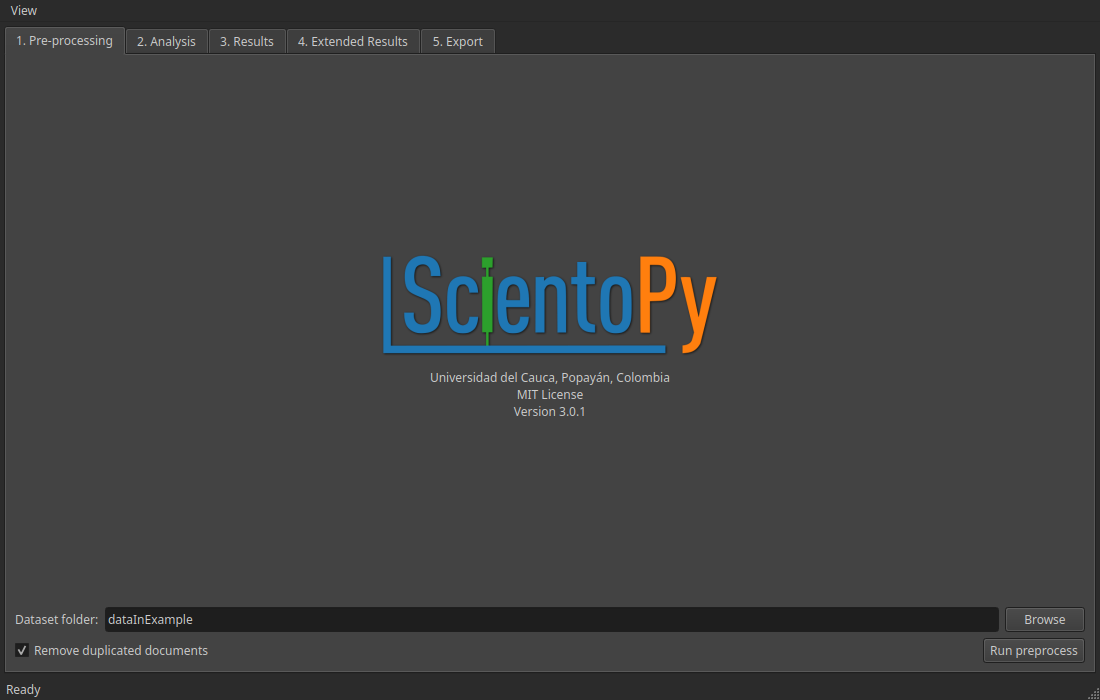
\includegraphics[width=0.85\textwidth]{./figures/gui_preprocess_tab.png}
\end{center}

\subsection{Menu bar}
\begin{itemize}
\item \textbf{View $\rightarrow$ Appearance:} Switch between Light, Dark, and System theme modes. The selected mode is saved and restored on next launch.
\end{itemize}

\subsection{Keyboard shortcuts}
\begin{itemize}
\item \textbf{Ctrl+O} -- Browse and select a dataset folder
\item \textbf{Ctrl+R} -- Run (preprocess on Tab 1, analysis on Tab 2)
\item \textbf{Ctrl+1/2/3/4/5} -- Switch to the corresponding tab
\item \textbf{Ctrl+C} -- Copy selected cells in the Results or Extended Results tables
\end{itemize}

\subsection{Status bar}
The status bar at the bottom of the window shows feedback messages such as ``Preprocessing complete -- 5,548 papers'', ``Analysis complete -- 10 topics found'', or error information.

\subsection{Configuration persistence}
ScientoPy saves the following settings to \verb|scientopy_config.json| and restores them on next launch: window size and position, splitter proportions, appearance mode, last dataset folder, and all analysis parameters (criterion, graph type, year range, topics length, skip first, window width, and checkbox states).


\section{Download the bibliometric dataset}
This section describes how to download the proper dataset from Scopus and WoS. Define a search criteria that will be used for Scopus and WoS. For this guide and for the example dataset we are using: ``Bluetooth low energy''.

\subsection{Download the dataset from Scopus}
\begin{enumerate}
\item Make your search with the defined search criteria for Article title, Abstract, Keywords.
\item Select all the results and click on Export:
	\begin{center}
		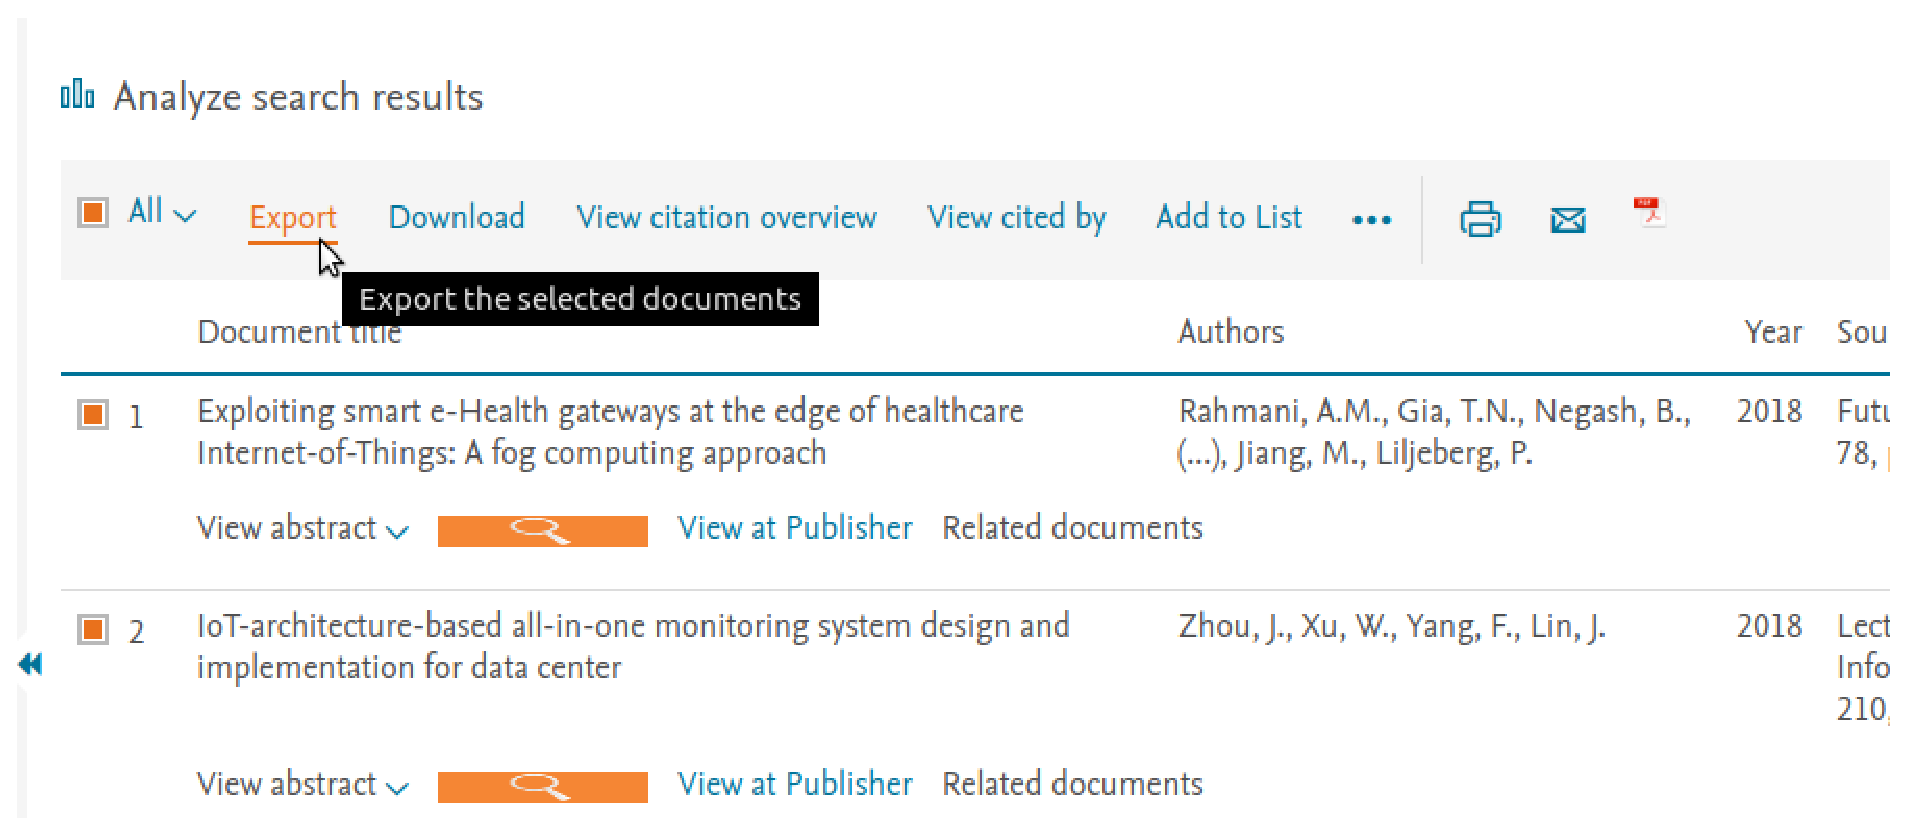
\includegraphics[scale=0.33]{./figures/scopus1.eps}
	\end{center}

\item Select as method of export \textbf{CSV (Excel)}, and select the Customize export \textbf{Citation information, Bibliographical information, Abstract and Keywords}, then click on Export:
	\begin{center}
		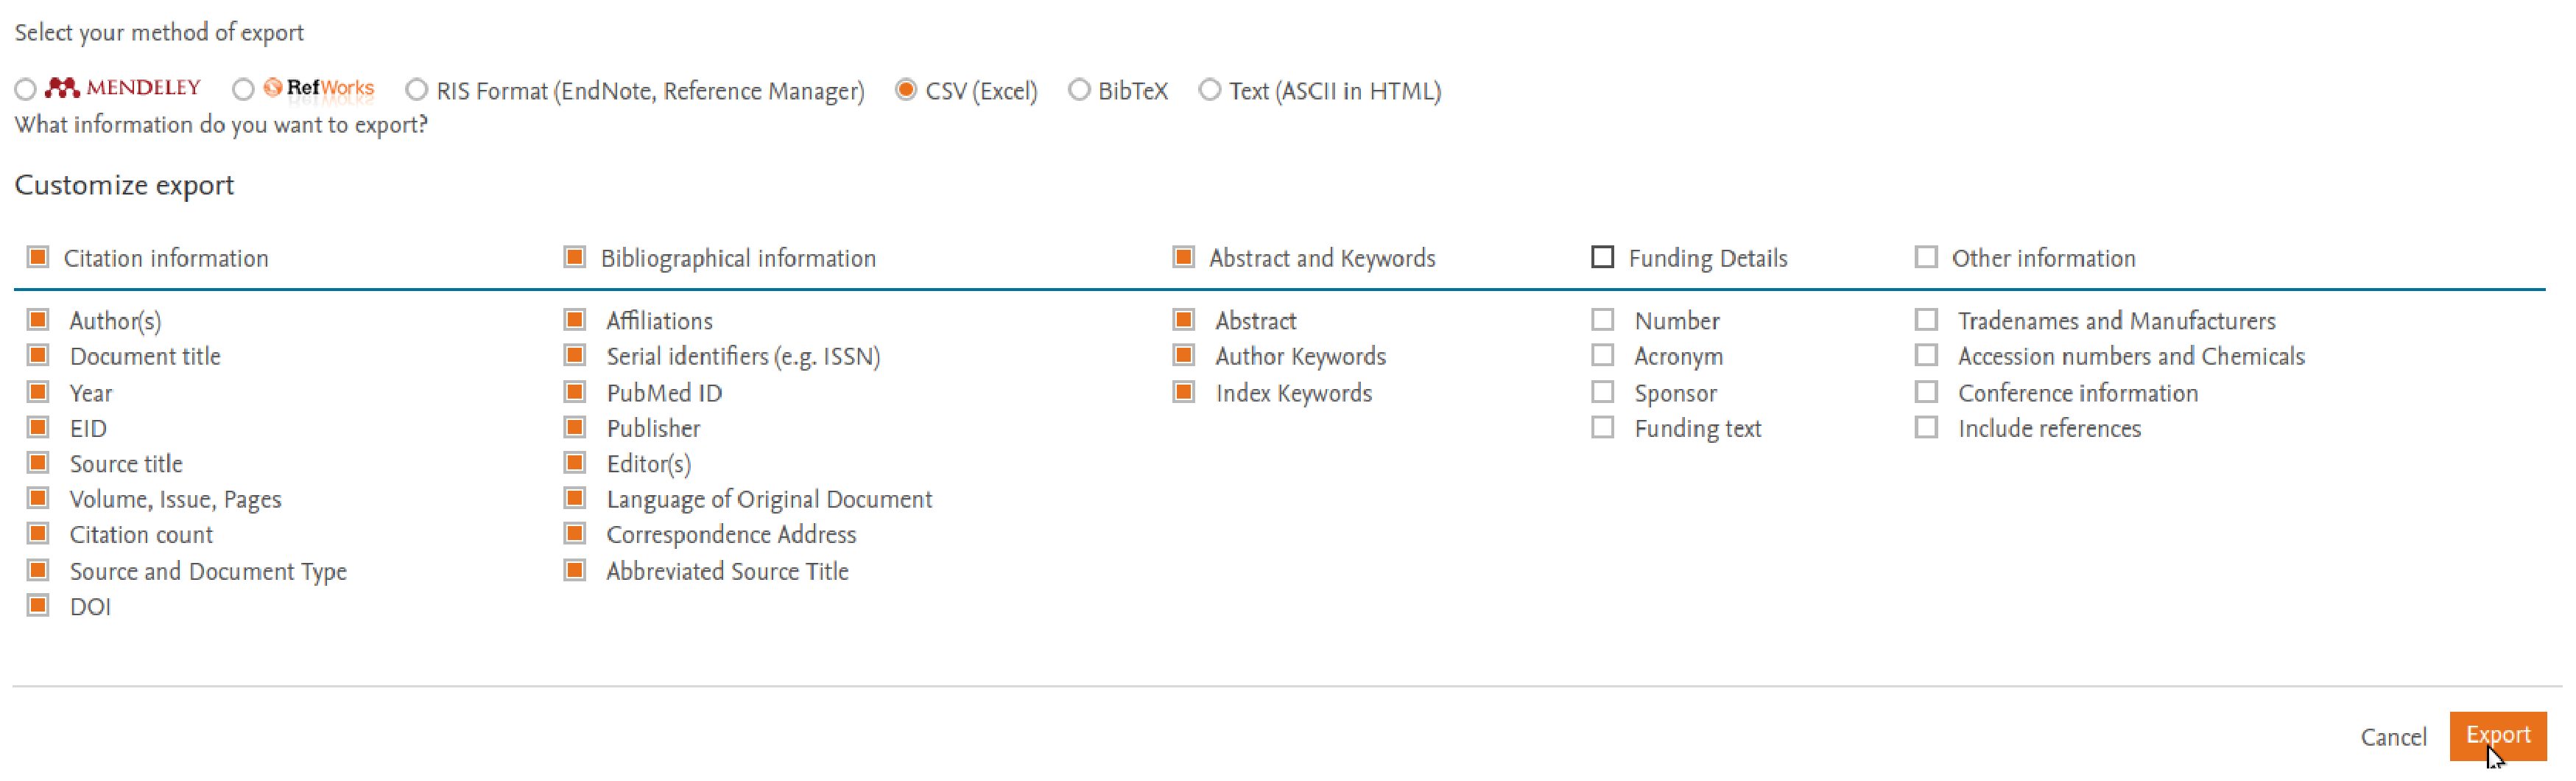
\includegraphics[scale=0.3]{./figures/scopus2.eps}
	\end{center}

\item Save the file on the dataset folder (e.g. \verb|/ScientoPy/dataIn|)
\end{enumerate}


\subsection{Download the dataset from WoS}
\begin{enumerate}
\item Make your search with the defined search criteria for Topic.
\item Select \textbf{Save in Other File Formats}
	\begin{center}
		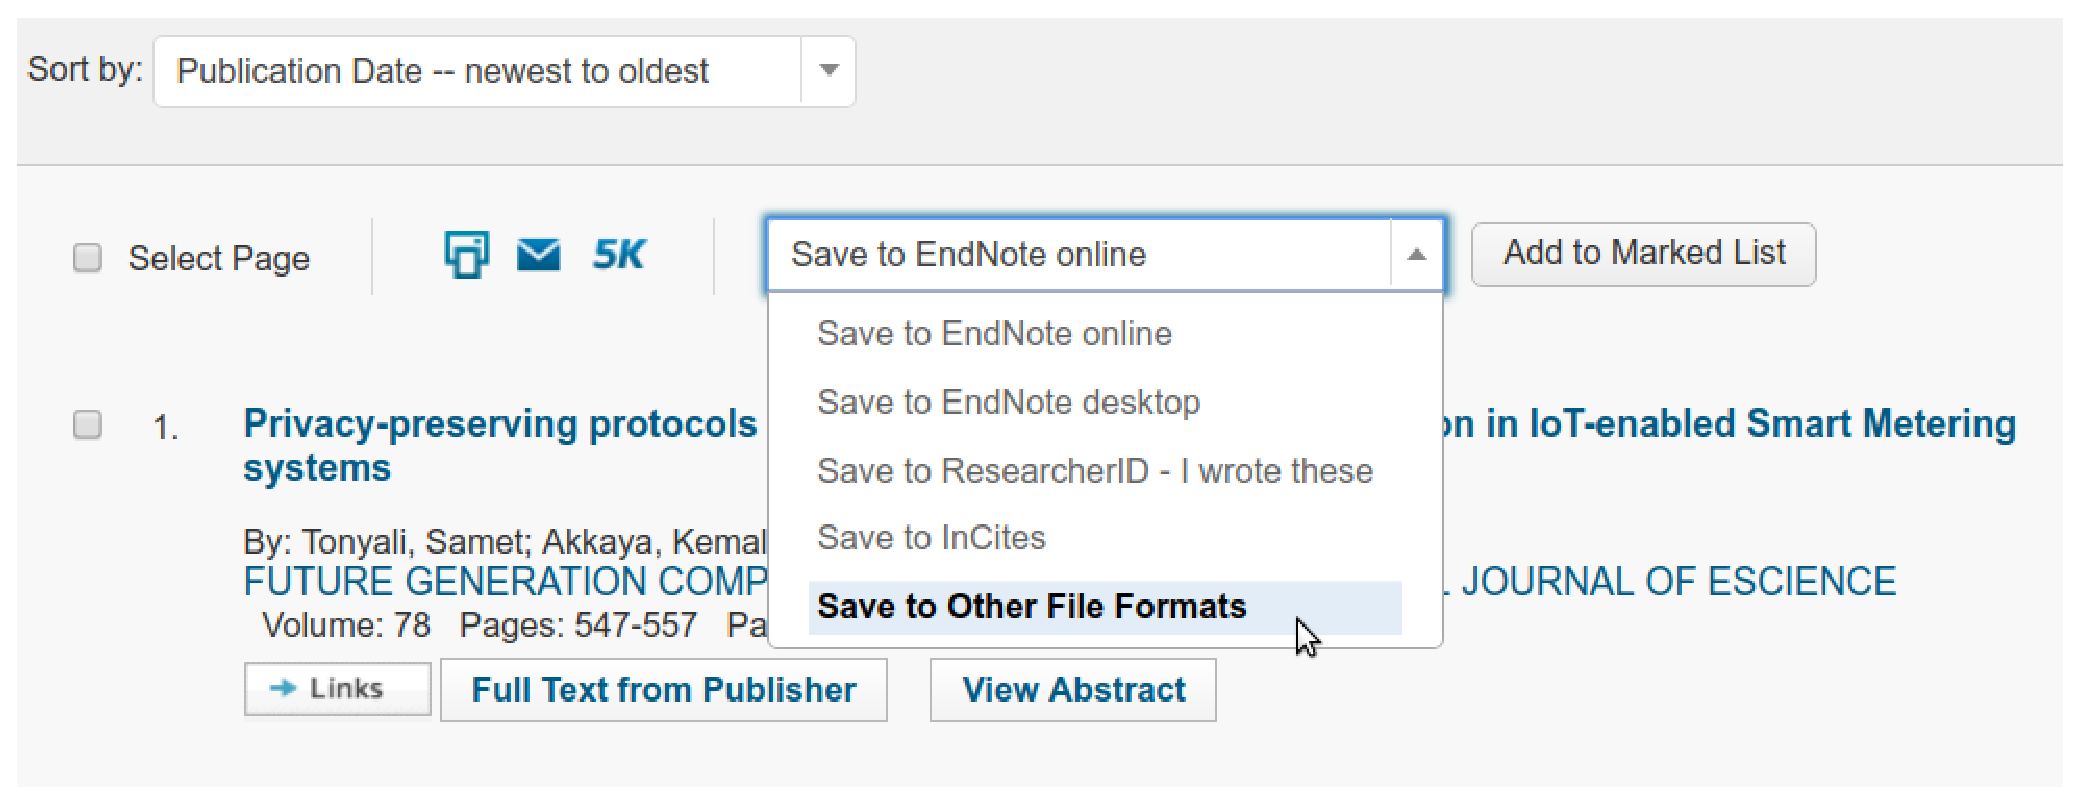
\includegraphics[scale=0.33]{./figures/wos1.eps}
	\end{center}

\item Select the number of records to download, on Record Content select \textbf{Full Record and Cited References}, on File Format select \textbf{Tab-delimited (Win, UTF-8)}, and click on Send.
	\begin{center}
		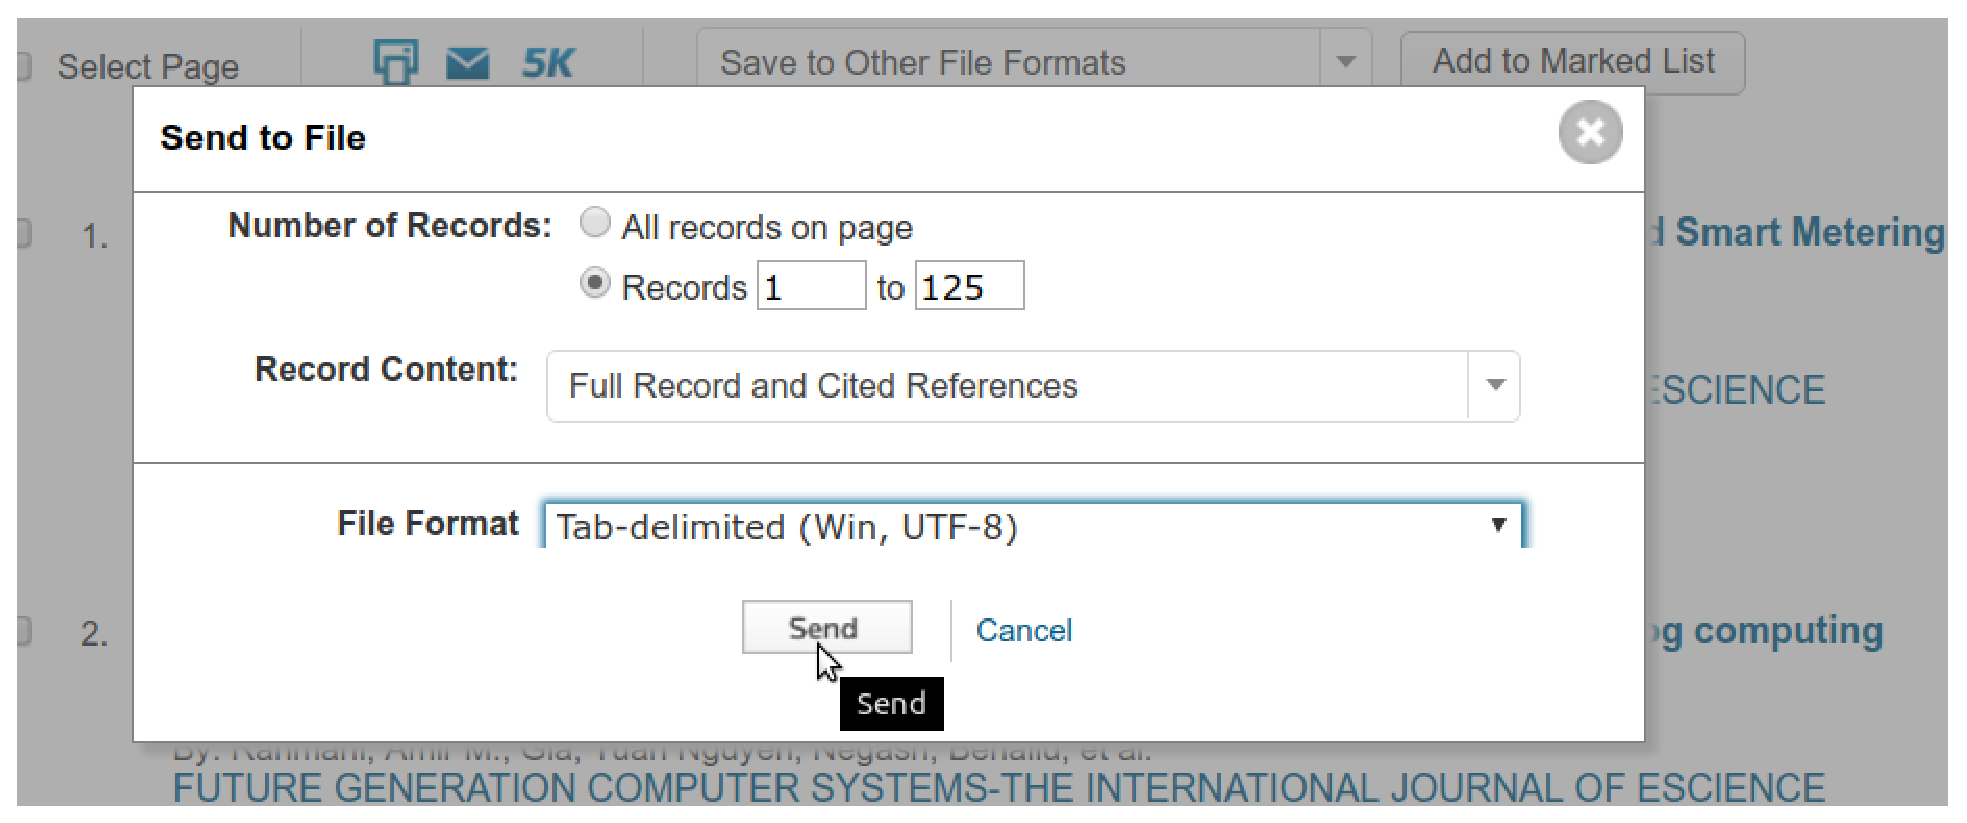
\includegraphics[scale=0.33]{./figures/wos2.eps}
	\end{center}

\item Save the file on the dataset folder (e.g. \verb|/ScientoPy/dataIn|)
\end{enumerate}


\section{Preprocessing (Tab 1)}

First we need to preprocess the downloaded dataset. This preprocess merges all the downloaded files from the dataset folder into a single file. Also, this process removes the duplicated documents. To preprocess the example dataset (``Bluetooth low energy'' located in \verb|dataInExample|), open ScientoPy and follow the next steps:

\begin{center}
	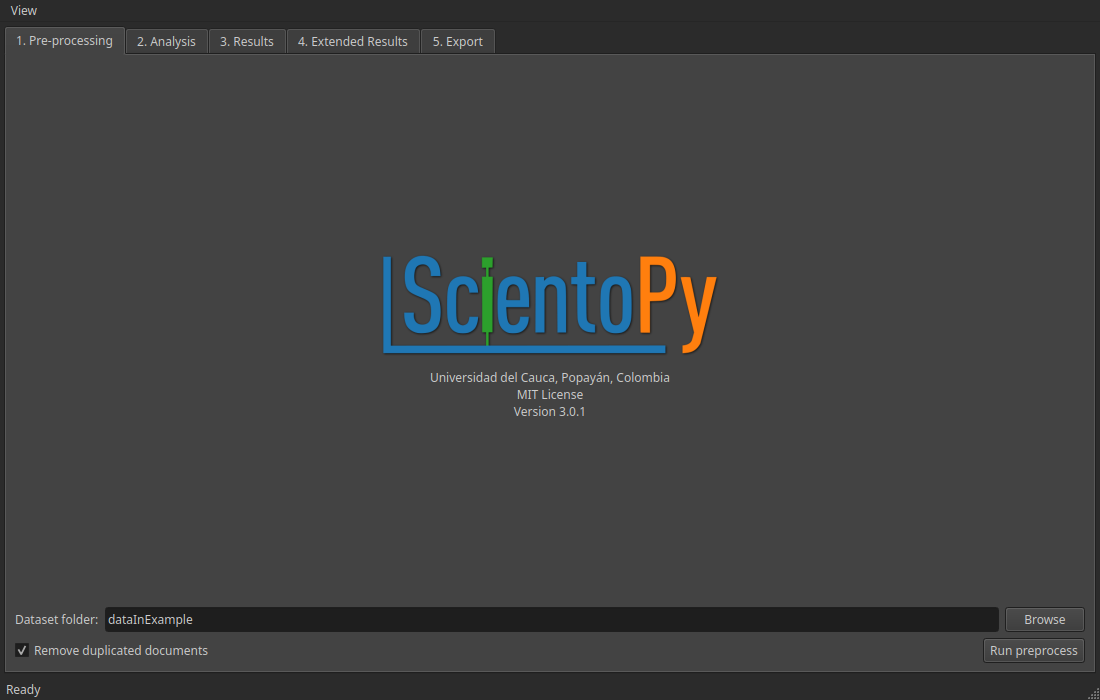
\includegraphics[width=0.85\textwidth]{./figures/gui_preprocess_tab.png}
\end{center}

\begin{enumerate}
\item Click the \verb|Browse| button, and select the folder that contains the downloaded dataset. The folder is scanned \textbf{recursively}, so Scopus and WoS exports can be placed in sub-directories. For the example dataset, select the folder \verb|dataInExample| inside the ScientoPy directory. Alternatively, use the keyboard shortcut \textbf{Ctrl+O}.
\item Ensure the \verb|Remove duplicated documents| checkbox is checked (default).
\item Click the \verb|Run preprocess| button (or press \textbf{Ctrl+R}). A progress dialog appears and shows each stage of the pipeline: \verb|[1/4] Loading papers|, \verb|[2/4] Disambiguating Scopus author names|, \verb|[3/4] Removing duplicates|, and \verb|[4/4] Saving preprocessed corpus|, with a progress bar per stage.
\item After preprocessing completes, the preprocess brief graph will appear and the application will automatically switch to the \textbf{3. Results} tab showing the preprocess brief table.
\end{enumerate}

As result, inside the folder \verb|ScientoPy/dataPre| you will find the following files:
\begin{itemize}
\item \textbf{papersPreprocessed.parquet:} canonical preprocessed corpus (Apache Parquet, Zstd-compressed). This is the input used by every subsequent analysis. To get a Scopus- or WoS-style CSV copy, use the \textbf{5. Export} tab (Section~\ref{sec_export_tab}).
\item \textbf{PreprocessedBrief.csv:} this file briefs the pre-process statistics results, such as duplicated papers removed, types of documents, and others.
\end{itemize}


\section{Analysis (Tab 2)}

The analysis tab lets you perform scientometric analysis operations. Click on the \verb|2. Analysis| tab to access it.

\begin{center}
	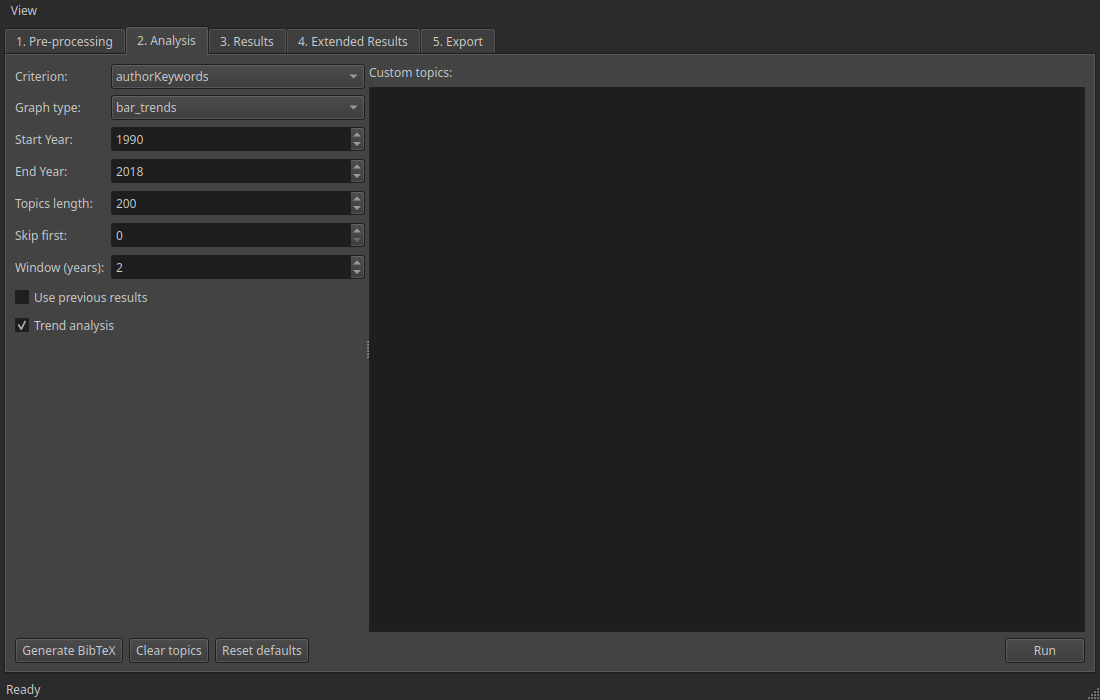
\includegraphics[width=0.85\textwidth]{./figures/gui_analysis_tab.png}
\end{center}

\subsection{Analysis parameters (left panel)}

\begin{itemize}
\item \textbf{Criterion:} the search criterion to analyze, such as author keywords, author names, countries, etc. See Table~\ref{table_criterion} for the full list.
\item \textbf{Graph type:} the type of output graph. See Section~\ref{sec_graph_types} for details.
\item \textbf{Start year:} limit the start year for the analysis and graphs.
\item \textbf{End year:} limit the end year for the analysis and graphs.
\item \textbf{Topics length:} number of top topics to find in the selected criterion.
\item \textbf{Skip first:} number of first top topics to skip during the analysis.
\item \textbf{Window (years):} window width in years for growth indicators (AGR, ADY).
\item \textbf{Use previous results:} run the analysis based on the output documents from the previous run.
\item \textbf{Trend analysis:} find the top trending topics with the highest average growth rate.
\end{itemize}

\subsection{Custom topics (right panel)}

The right panel contains a text area for entering custom topics. Enter one topic per line. Topics can be grouped with commas and separated by line breaks. The asterisk (*) wildcard is supported. See Section~\ref{sec_custom_topics} for details.

\subsection{Action buttons (bottom bar)}

\begin{itemize}
\item \textbf{Generate BibTeX:} generate a BibTeX bibliography file from a LaTeX document (see Section~\ref{sec_bibtex}).
\item \textbf{Clear topics:} clear the Custom topics text area.
\item \textbf{Reset defaults:} reset all analysis parameters to their default values (criterion: authorKeywords, graph type: bar\_trends, years: 1990 to last year, topics length: 10, skip first: 0, window: 2, checkboxes unchecked, custom topics cleared).
\item \textbf{Run:} execute the analysis with the current parameters. Can also be triggered with \textbf{Ctrl+R}.
\end{itemize}

After the analysis completes, results are displayed in the \textbf{3. Results} and \textbf{4. Extended Results} tabs, and the output graph appears.

\subsection{Criterion descriptions}

The ScientoPy criterion are described in Table~\ref{table_criterion}:

\begin{table}[h]
	\centering
	\caption{ScientoPy criterion description}
	\label{table_criterion}

	\renewcommand{\arraystretch}{1.5}
	\begin{tabular}{p{3.5cm} p{10cm}}
	\hline\noalign{\smallskip}
	Criterion       & Description                             \\
	\noalign{\smallskip}\hline\noalign{\smallskip}
	\textbf{author}         & Authors last name and first name initial                                                                       \\
	\textbf{sourceTitle}    & Publication or journal name                                                                                    \\
	\textbf{subject}        & Research areas, only from WoS documents                                                                        \\
	\textbf{authorKeywords} & Author keywords                                                                                                \\
	\textbf{indexKeywords}  & Keywords generated by the index, from WoS \textit{Keyword Plus}, and from Scopus \textit{Indexed keywords} \\
	\textbf{bothKeywords}   & AuthorKeywords and indexKeywords are used for this search                                                      \\
	\textbf{abstract}       & Document abstract, for use with pre-defined topics and asterisk wildcard\\
	\textbf{documentType}   & Type of document                                                                                               \\
	\textbf{dataBase}       & Database where the document was extracted (WoS or Scopus)                                                      \\
	\textbf{country}        & Country extracted from authors affiliations                                                                    \\
	\textbf{institution}    & Institution extracted from authors affiliations                                                                \\
	\textbf{institutionWithCountry}    & Institution with country extracted from authors affiliations                                        \\
	\noalign{\smallskip}\hline
	\end{tabular}

\end{table}

\subsection{Extract top topics}

To find the top 10 author keywords, keep the default parameters in the analysis tab and click the \verb|Run| button. This will generate a list with the top 10 topics on the selected criterion (in this case authorKeywords), with the number of documents per topic. The bar trends graph will appear, and the quantitative results are saved in the folder \verb|ScientoPy/results| and displayed in the \textbf{3. Results} tab.

\subsection{Analyze custom topics inside a criterion}
\label{sec_custom_topics}

If you want to analyze custom topics, such as comparing two countries' publication trends, enter the topics in the \verb|Custom topics| text area (one topic per line):

\begin{center}
	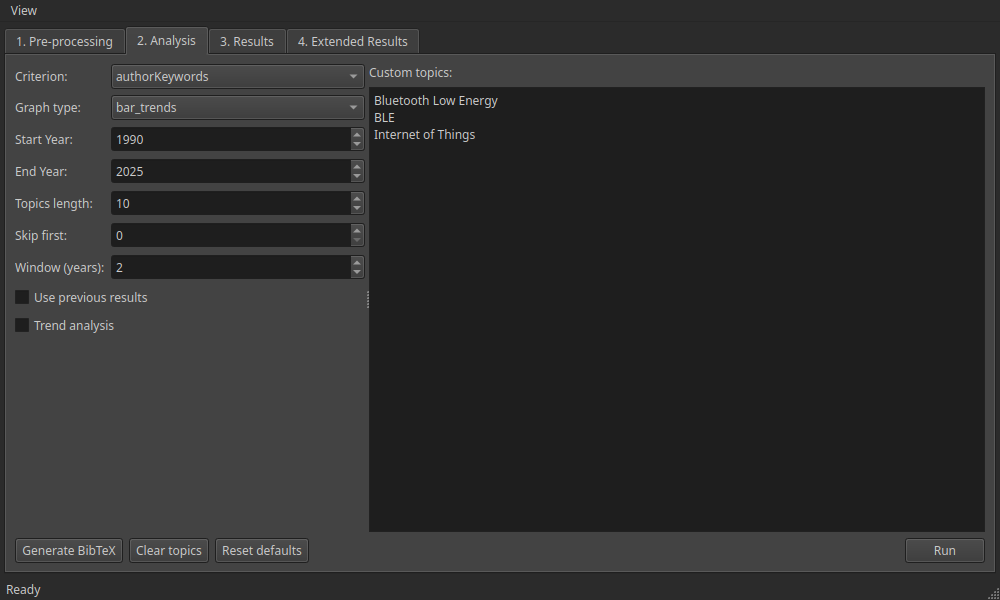
\includegraphics[width=0.85\textwidth]{./figures/gui_analysis_custom_topics.png}
\end{center}

You can analyze any topic in any criterion. You can also group two or more topics into one by separating them with commas. This is useful for abbreviations and plural/singular forms, for example:
\begin{verbatim}
WSN, Wireless sensor network, Wireless sensor networks
RFID, RADIO FREQUENCY IDENTIFICATION
\end{verbatim}

\textbf{Tip:} You can also use the \verb|Analyze selection| button in the \textbf{3. Results} tab to copy selected topic names directly into the Custom topics field (see Section~\ref{sec_results_tab}).

\subsection{Asterisk (*) wildcard}

You can use the asterisk wildcard to find phrases or words which start or end with the entered text. For example, entering \verb|device*| in the Custom topics area will match ``device'', ``devices'', ``device integration'', etc.

ScientoPy prints the topics found for the wildcard-based search in the console output. You can copy this information to analyze each specific topic found individually.

\subsection{Evolution plot}

Select \verb|evolution| as the Graph type to see an evolution plot. This option plots the accumulative documents, average documents per year (ADY), and percentage of documents in the last years (PDLY).

\textbf{Note:} select the right start and end year limits that fit your plot lines best.

\subsection{Finding trending topics}

ScientoPy can find the top trending topics based on the highest average growth rate (AGR). The AGR is calculated using the following equation:
\begin{equation*}
AGR = \frac{\sum\limits_{i = Y_s}^{Y_e}P_i - P_{i-1}}{(Y_e - Y_s)+1},
\label{equation_AGR}
\end{equation*}

\setlength{\leftskip}{5cm}
\hspace*{-1cm}where:\\
$AGR$ = Average growth rate;\\
$Y_s$ = Start year;\\
$Y_e$ = End year;\\
$P_i$ = Number of publications on year $i.$\\

\setlength{\leftskip}{0pt}

To find the top trending topics, check the \verb|Trend analysis| checkbox and click \verb|Run|. ScientoPy will find the top 200 topics, calculate the AGR for the specified window period, and sort them from highest to lowest AGR.

\subsection{Analysis based on the previous results}

ScientoPy generates a lightweight internal file with all the output documents from the last run so that subsequent analyses can chain off it. For example, if you run an analysis with criterion \verb|country| and custom topic \verb|Canada|, ScientoPy writes \verb|results/lastAnalysis.parquet| with every document whose authors are affiliated in Canada. In previous versions this file was a CSV called \verb|results/papersPreprocessed.csv|; analyses no longer write any CSV automatically. Use the \textbf{5. Export} tab (Section~\ref{sec_export_tab}) if you need a CSV copy.

This output file can be used as input for a subsequent analysis by checking the \verb|Use previous results| checkbox. For example, you could then select criterion \verb|authorKeywords| to find the top author keywords from Canadian papers, or select criterion \verb|country| to find which countries have the most co-authored documents with Canada.

\textbf{Note:} the output documents file is only generated when \verb|Use previous results| is \textbf{not} checked. Running multiple analyses with this option checked will not overwrite the documents output file.


\section{Results tab (Tab 3)}
\label{sec_results_tab}

The Results tab displays the analysis output in a sortable table. After running a preprocess, it shows the preprocessing brief. After running an analysis, it shows the top topics with their statistics (Total, AGR, ADY, PDLY, h-index, and documents per year).

\begin{center}
	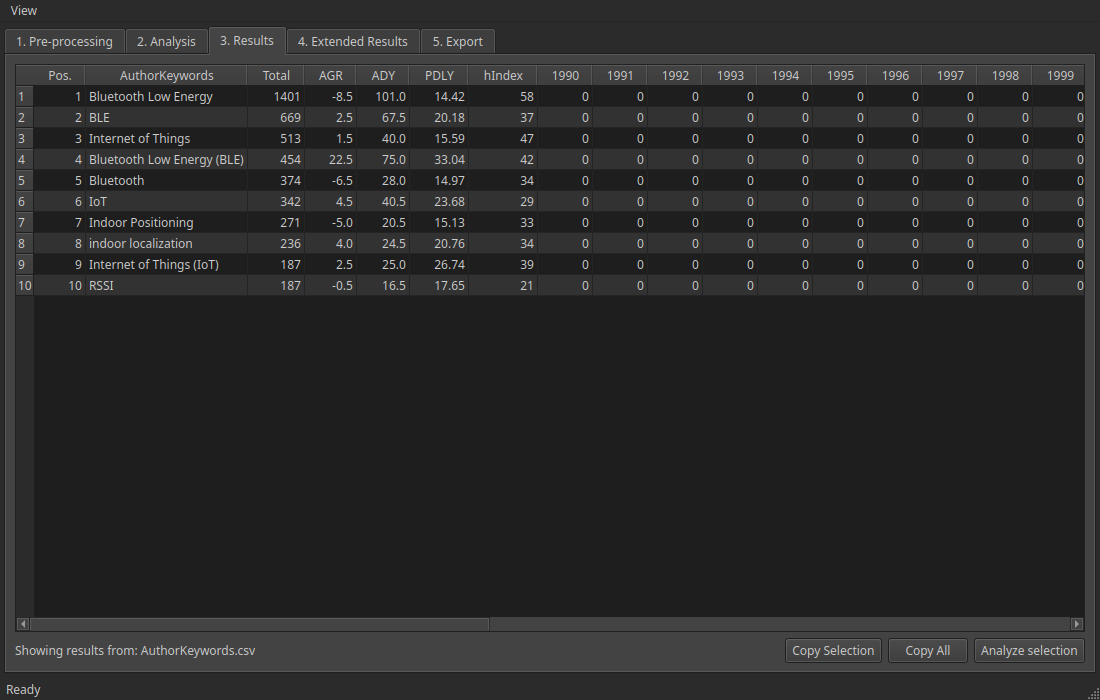
\includegraphics[width=0.85\textwidth]{./figures/gui_results_tab.png}
\end{center}

\subsection{Column tooltips}
Hover over column headers to see tooltips with definitions of abbreviations:
\begin{itemize}
\item \textbf{AGR:} Average Growth Rate -- mean year-over-year change in publications within the window period.
\item \textbf{ADY:} Average Documents per Year -- mean publications per year within the window period.
\item \textbf{PDLY:} Percentage of Documents in Last Years -- proportion of total documents published within the window period.
\item \textbf{hIndex:} h-index -- the largest number $h$ such that $h$ documents have at least $h$ citations each.
\end{itemize}

\subsection{Action buttons}

\begin{itemize}
\item \textbf{Copy Selection:} copy the selected cells to the clipboard (also available via Ctrl+C).
\item \textbf{Copy All:} copy the entire table to the clipboard.
\item \textbf{Analyze selection:} copy the topic names from the selected rows to the \verb|Custom topics| text area in the Analysis tab, and switch to the Analysis tab. This is useful for quickly selecting topics from the results for further analysis with a different graph type or criterion.
\end{itemize}


\section{Extended Results tab (Tab 4)}

The Extended Results tab shows the detailed per-document output after running an analysis. Each row represents a paper associated with one of the analyzed topics, including authors, title, year, source, citations, DOI, and other metadata.

\begin{center}
	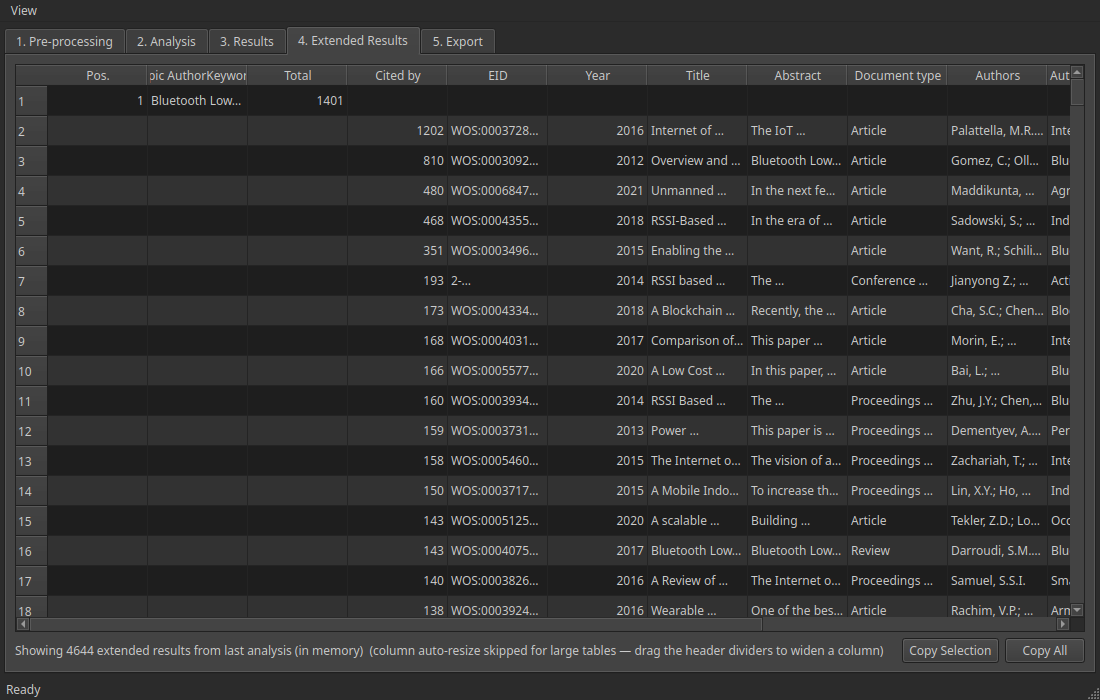
\includegraphics[width=0.85\textwidth]{./figures/gui_ext_results_tab.png}
\end{center}

The table is sortable by clicking column headers and supports cell selection with Ctrl+C copy.

\subsection{Action buttons}

\begin{itemize}
\item \textbf{Copy Selection:} copy the selected cells to the clipboard.
\item \textbf{Copy All:} copy the entire table to the clipboard.
\end{itemize}


\section{Export tab (Tab 5)}
\label{sec_export_tab}

The Export tab produces on-demand Scopus- or WoS-style CSV files from either the full preprocessed corpus or the most recent analysis results. Exports are opt-in: neither preprocessing nor analysis writes CSV by itself anymore (the canonical on-disk format is Parquet, which is much smaller and loads faster).

\begin{center}
	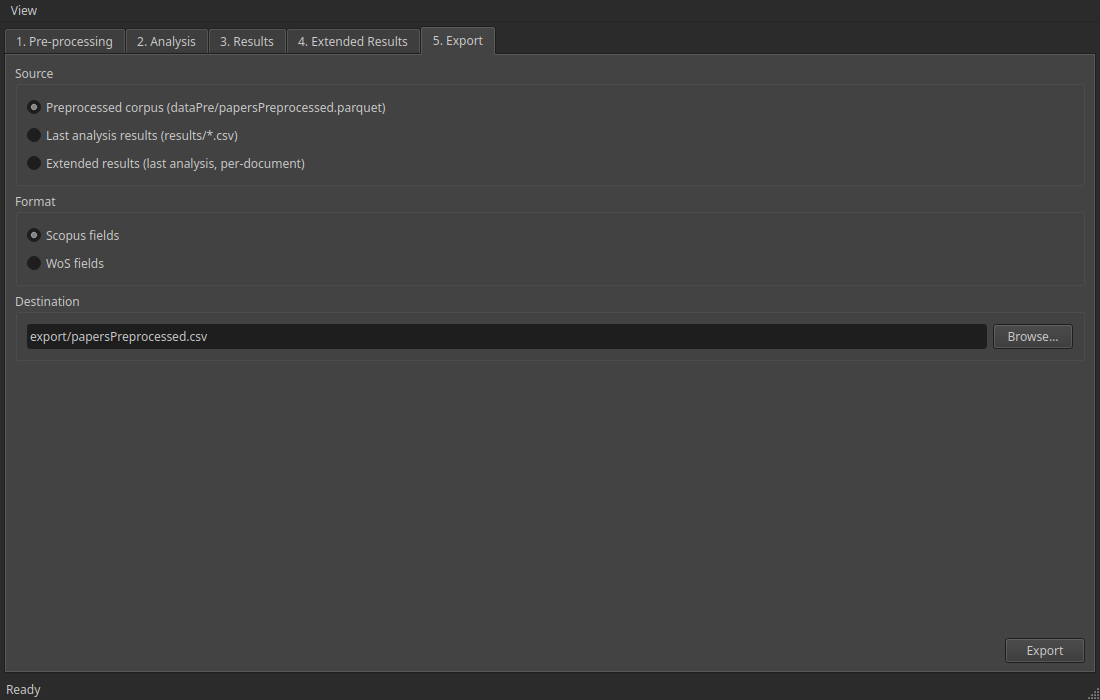
\includegraphics[width=0.85\textwidth]{./figures/gui_export_tab.png}
\end{center}

\begin{enumerate}
\item \textbf{Source.}
	\begin{itemize}
	\item \textbf{Preprocessed corpus} -- export \verb|dataPre/papersPreprocessed.parquet| as a single CSV.
	\item \textbf{Last analysis results} -- copy all CSVs currently under \verb|results/| into the chosen destination folder.
	\item \textbf{Extended results (last analysis, per-document)} -- write the detailed per-document \verb|*_extended.csv| for the analysis that is still in memory from the last \verb|Run|. This file is no longer produced automatically because it can reach hundreds of thousands of rows on large corpora. The option is disabled until you have run an analysis in the current session.
	\end{itemize}
\item \textbf{Format.} Only applies to \emph{Preprocessed corpus}; greyed out for the other sources.
	\begin{itemize}
	\item \textbf{Scopus fields} -- Scopus column-naming convention (\verb|Authors|, \verb|Title|, \verb|EID|, \ldots).
	\item \textbf{WoS fields} -- Web of Science field tags (\verb|AU|, \verb|TI|, \verb|UT|, \ldots).
	\end{itemize}
\item \textbf{Destination.} A file path for Preprocessed corpus (default \verb|export/papersPreprocessed.csv|) or Extended results (default \verb|export/<Criterion>_extended.csv|), or a folder path for Last analysis results (default \verb|export/results/|). Use the \verb|Browse...| button to pick an alternative path.
\item \textbf{Export.} Click the \verb|Export| button. A progress dialog appears and updates through the stages \verb|Reading preprocessed corpus...| and \verb|Writing CSV (scopus fields)| with a live 0\%--100\% bar during the write. On completion, a confirmation dialog offers an \verb|Open| button to reveal the output file or folder.
\end{enumerate}

The \verb|Export| button is automatically disabled when the chosen Source has nothing to export (e.g.\ no preprocessed corpus has been produced yet, or \verb|results/| is empty). The same export functionality is available from the command line via \verb|exportPapers.py| (run \verb|python3 exportPapers.py -h| for the full list of options).


\section{Generate BibTeX}
\label{sec_bibtex}

With ScientoPy you can generate a \LaTeX{} BibTeX file for your references. Follow the next steps:

\begin{enumerate}
\item Run an analysis to generate results.
\item Open the Extended Results tab (Tab 4) and find the EID values of the papers you want to cite.
\item In your LaTeX document, use the paper EID values as citation keys inside \verb|\cite{}| commands, for example: \verb|\cite{2-s2.0-85012345678}|
\item Save your LaTeX document.
\item In the Analysis tab, click the \verb|Generate BibTeX| button and select the LaTeX document.
\item ScientoPy will find all EID citation keys in the document and generate a BibTeX file with the corresponding bibliographic entries. The output file is saved next to the input file as \verb|<filename>_bibliography.bib|.
\end{enumerate}

\textbf{Note:} for your reference we have included an article LaTeX file example in \verb|latexExample/article_example.tex|. This contains cites from the example dataset. To test the Generate BibTeX capability:
\begin{itemize}
\item Preprocess the example dataset located in \verb|dataInExample|
\item In the Analysis tab, click \verb|Generate BibTeX|
\item Select the file \verb|latexExample/article_example.tex|
\item Compile the LaTeX file with: \verb|latexmk -pdf article_example.tex|
\end{itemize}


\section{Output files and directories}

After running ScientoPy analysis you will find the following folder and files structure:

\vspace*{0.5cm}
\dirtree{% This % is required
	.1 ScientoPy.
	.2 dataInExample.
	.2 dataPre.
	.3 papersPreprocessed.csv.
	.3 PreprocessedBrief.csv.
	.2 graphs.
	.2 latexExample.
	.2 Manual.
	.2 results.
	.3 AuthorKeywords.csv.
	.3 AuthorKeywords\_extended.csv.
	.3 papersPreprocessed.csv.
	.2 scientopy\_config.json.
}

These folders and output files are described below:

\begin{itemize}
	\item \textbf{dataInExample:} contains Scopus and WoS example data set for the search criteria ``Bluetooth low energy'' downloaded on April 2, 2026. This is the input example for preprocessing.

	\item \textbf{dataPre:} output folder for the preprocessing results, and input folder for the analysis.

	\item \textbf{papersPreprocessed.csv:} preprocessed papers data with all input documents merged, filtered, and duplicates removed. This is the input file that the analysis uses.

	\item \textbf{PreprocessedBrief.csv:} preprocessing brief table that shows the preprocessing results related to total papers found per database, the omitted papers, the duplicated papers count per database, and the total number of papers per paper type (Conference paper, article, review...).

	\item \textbf{graphs:} graphs output folder for preprocessing and analysis.

	\item \textbf{latexExample:} folder with the LaTeX file article example to generate the BibTeX from the preprocessed dataset.

	\item \textbf{Manual:} folder with the PDF manual.

	\item \textbf{results:} output folder for analysis result files.

	\item \textbf{AuthorKeywords.csv:} analysis output file for the selected criterion (in this case authorKeywords) that shows the top or custom topics with the total number of documents, the Average Growth Rate (AGR), the Average Documents per Year (ADY), the Percentage of Documents in Last Years (PDLY), the h-index, and the documents per each year.

	\item \textbf{AuthorKeywords\_extended.csv:} analysis output file for the selected criterion that shows the top or custom topics with the documents related to each one.

	\item \textbf{papersPreprocessed.csv:} inside the results folder, this file contains the output papers from the last analysis run. This is used as input when the option \verb|Use previous results| is checked.

	\item \textbf{scientopy\_config.json:} user configuration file storing window geometry, appearance mode, and analysis parameters. Automatically created and updated.
\end{itemize}

\newpage
\section{ScientoPy graph types}
\label{sec_graph_types}

ScientoPy has 5 different ways to graph the results described on Table~\ref{table_graph_types}.

\begin{table}[!h]
	\centering
	\caption{ScientoPy output graph types}
	\label{table_graph_types}

	\renewcommand{\arraystretch}{1.5}
	\begin{tabular}{ p{4cm} p{3cm} p{10cm}}
	\hline\noalign{\smallskip}
	Graph type     &  Abbreviation & Description                             \\
	\noalign{\smallskip}\hline\noalign{\smallskip}
	Time line      & \verb|time_line| & Graphs the number of documents of each topic vs the publication year \\
	Horizontal bars  & \verb|bar| & Graphs the total number of documents of each topic in horizontal bars \\
	Horizontal bars trends  & \verb|bar_trends| & Graphs the total number of documents of each topic in horizontal bars, with the percentage of documents published in the last years \\
	Evolution     & \verb|evolution| & Graphs two plots, one with the accumulative number of documents vs the publication year, and another with the average papers per year vs the percentage of documents in the last years\\
	Word cloud     & \verb|word_cloud| & Generate a word cloud based on the topic total number of publications \\
	\noalign{\smallskip}\hline
	\end{tabular}
\end{table}

Below are some examples of these graph types.

\subsection{Time line graph}
\begin{center}
	
\includegraphics[width=0.75\textwidth]{./figures/graph_time_line.eps}
\end{center}

\subsection{Horizontal bars graph}
\begin{center}
	
\includegraphics[width=0.75\textwidth]{./figures/graph_bar.eps}
\end{center}

\subsection{Horizontal bars trends}

\begin{center}
	
\includegraphics[width=0.75\textwidth]{./figures/graph_bar_trends.eps}
\end{center}

\subsection{Evolution graph}

\begin{center}
	
\includegraphics[width=0.75\textwidth]{./figures/graph_evolution.eps}
\end{center}


\subsection{Word cloud graph}

\begin{center}
	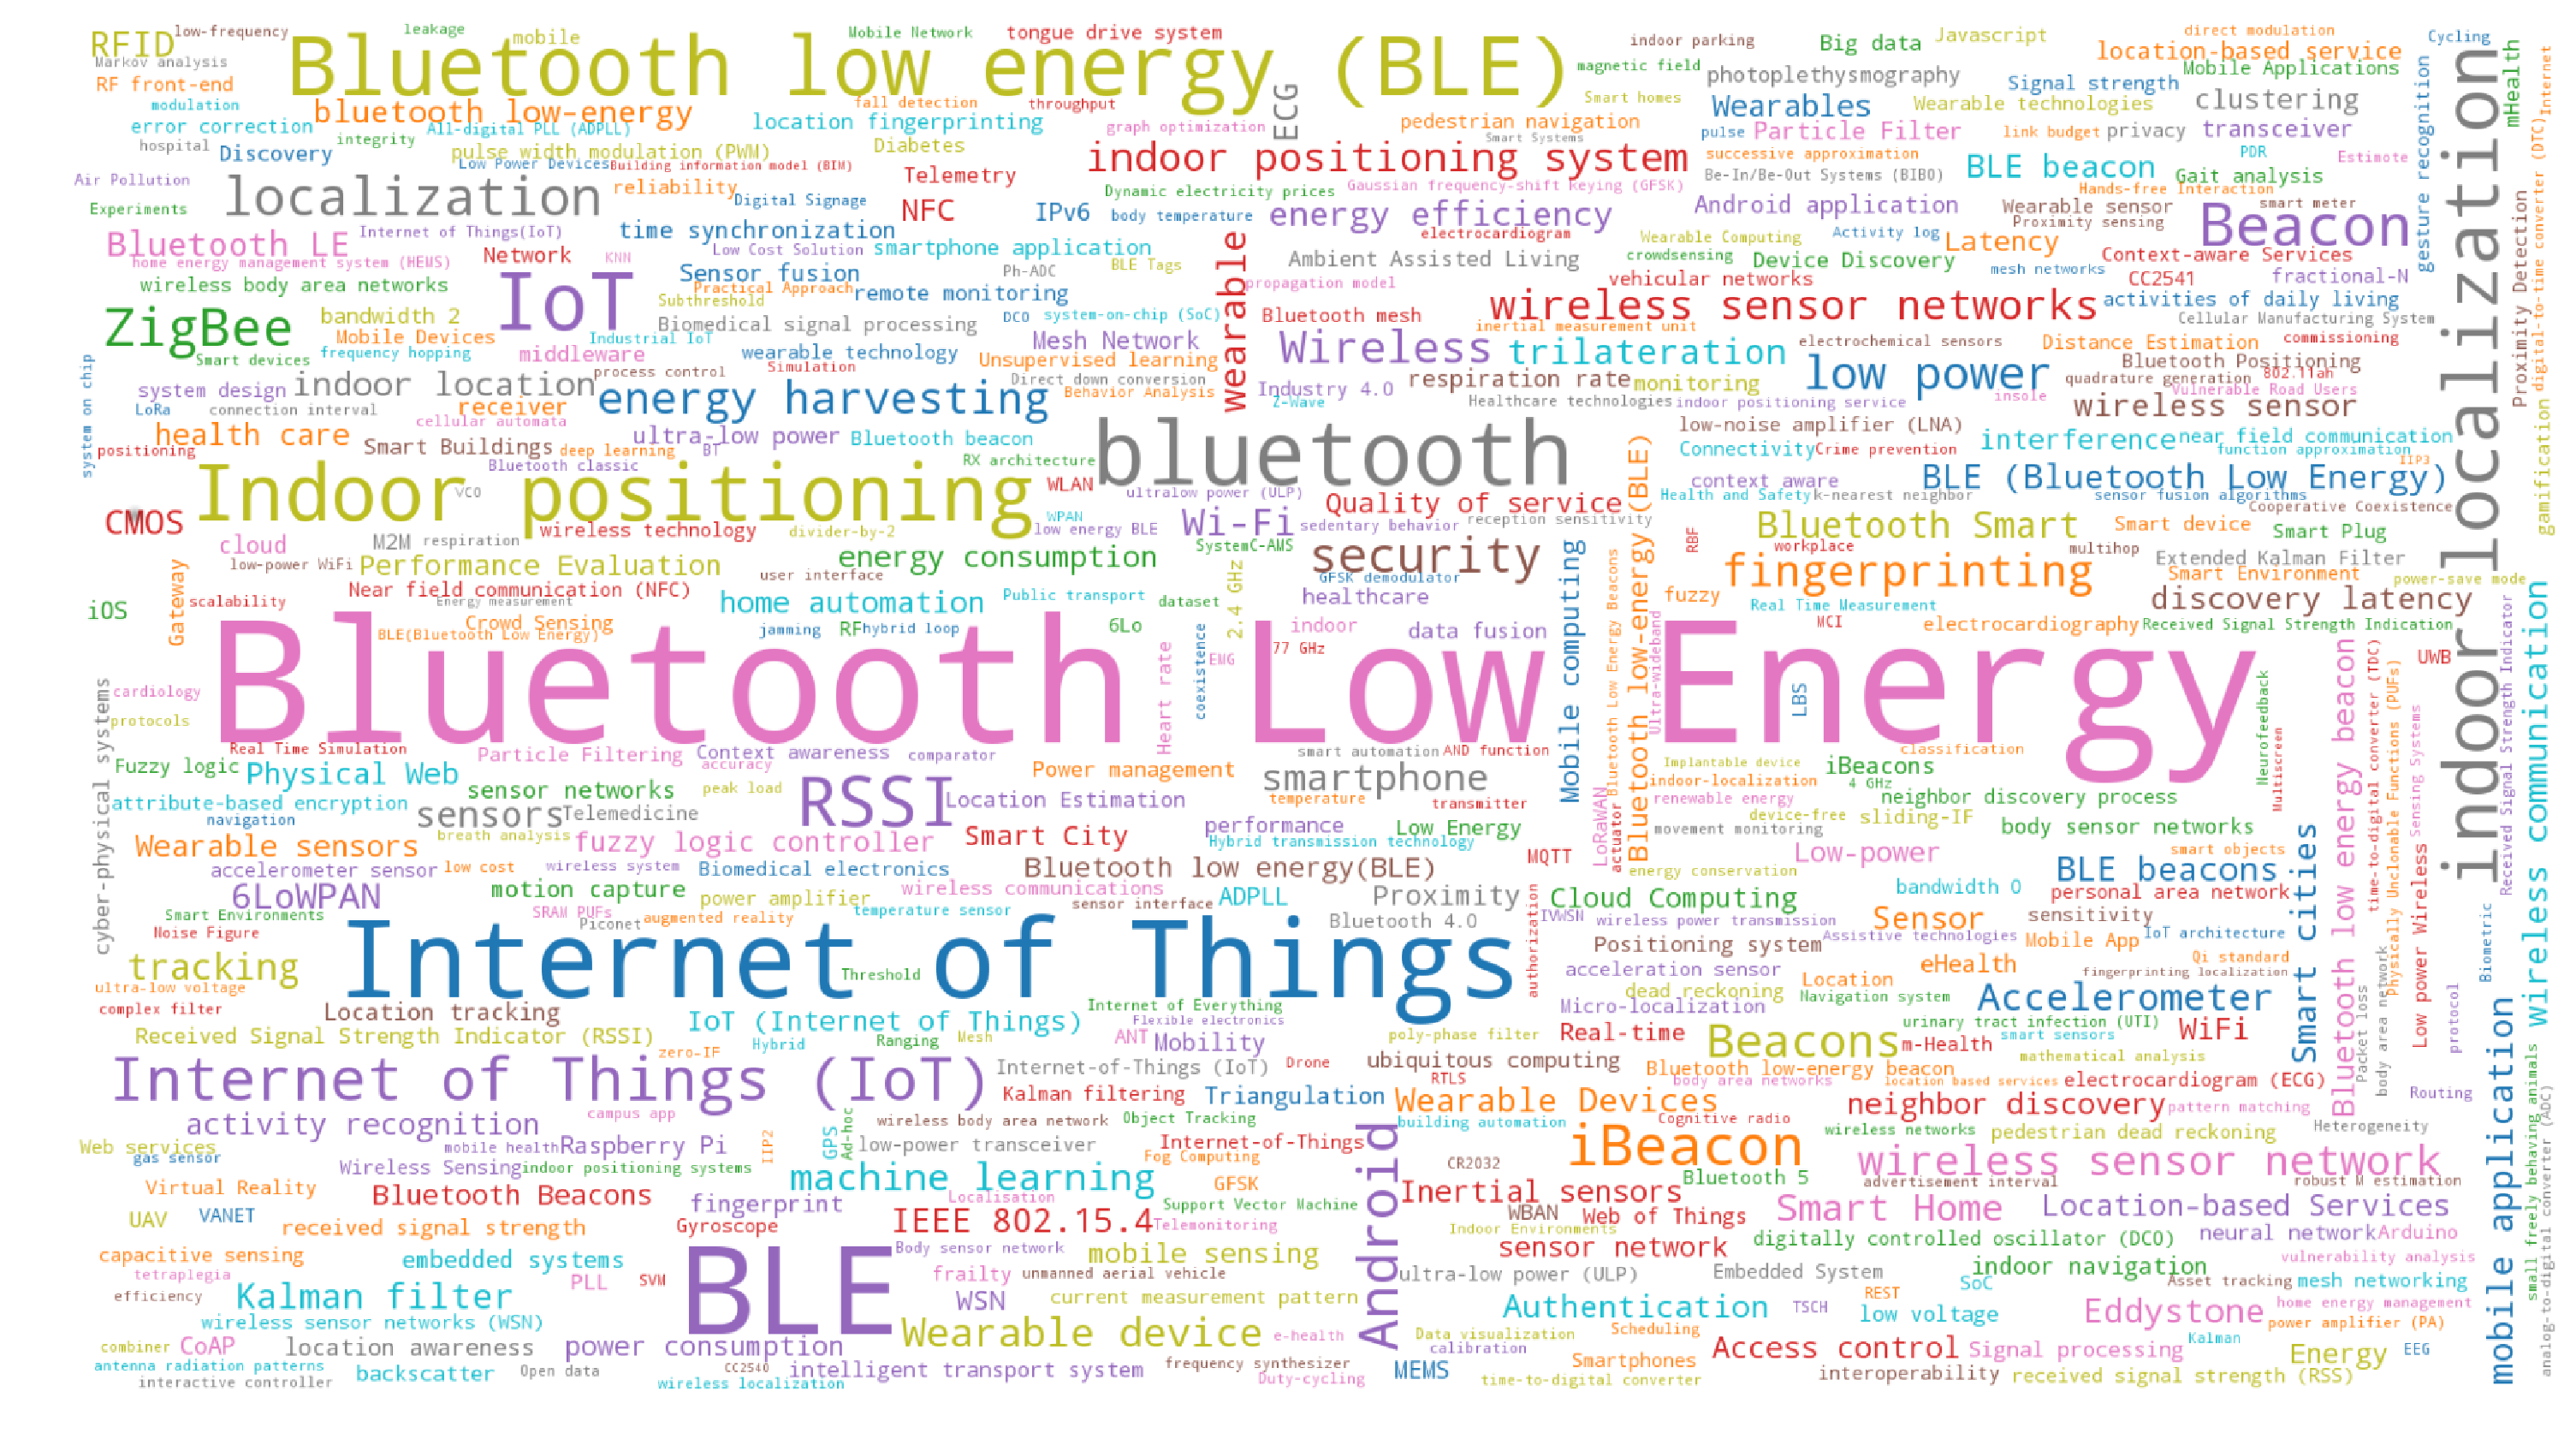
\includegraphics[width=0.9\textwidth]{./figures/graph_word_cloud.eps}
\end{center}


\end{document}
